
%***************************************************************************
%
% CreditCruncher - A portfolio credit risk valorator
% Copyright (C) 2003-2009 Gerard Torrent
%
% This program is free software; you can redistribute it and/or
% modify it under the terms of the GNU General Public License
% as published by the Free Software Foundation; either version 2
% of the License.
%
% This program is distributed in the hope that it will be useful,
% but WITHOUT ANY WARRANTY; without even the implied warranty of
% MERCHANTABILITY or FITNESS FOR A PARTICULAR PURPOSE.  See the
% GNU General Public License for more details.
%
% You should have received a copy of the GNU General Public License
% along with this program; if not, write to the Free Software
% Foundation, Inc., 59 Temple Place - Suite 330, Boston, MA 02111-1307, USA.
%
%***************************************************************************

\documentclass[a4paper,12pt,final]{article}
\usepackage{times}
\usepackage{latexsym}
\usepackage{amssymb}
\usepackage{abstract}
\usepackage[dvips]{graphicx}
\usepackage[american]{babel}
\usepackage[final]{listings}
\usepackage{fancyhdr}
\usepackage[flushmargin]{footmisc}
\usepackage{placeins}
\usepackage{verbatim}

%-----------------------------------------------------
% defining some useful values
%-----------------------------------------------------
\def\numversion{1.4}
\def\svnversion{R494}

%-----------------------------------------------------
% some format directives
%-----------------------------------------------------
\sloppy
\pagestyle{fancy}
\setlength\parindent{0ex}

%-----------------------------------------------------
% finally, the doc begins here
%-----------------------------------------------------
\begin{document}

\title{CreditCruncher - Technical Document}
\author{Gerard Torrent Gironella\\\\Version \numversion\ -\ \svnversion}
\date{}
\maketitle


%===========================================================================
\begin{abstract}
The ccruncher goal is to compute the credit risk of a portfolio, where 
investments are fixed income assets, taking into account default correlations
between economic sectors. This is done by determining the probability distribution 
of portfolio loss at time $T$ using the Monte Carlo method and computing the
usual risk statistics (Expected Loss, Standard Deviation, Value at Risk, Expected 
Shortfall).
\newline
\newline
\textbf{Keywords}: credit risk, Monte Carlo, gaussian copula, t-Student copula,
value at risk, expected shortfall.
\end{abstract}
\newpage


%===========================================================================
\tableofcontents
\newpage


%===========================================================================
\begin{comment}
\section{Introduction}

%TODO: Little schema how ccruncher solves problem (Monte Carlo, Copula, Portfolio, etc.)

\subsection{Alternatives}

\subsubsection{CreditRisk+ approach}
%TODO: fill this section

\subsubsection{CreditMetrics approach}
%TODO: fill this section

\subsubsection{Copula approach}
%TODO: fill this section

\subsection{Comparison}
%TODO: Comparison with other methods (CreditRisk+, CreditMetrics)
%TODO: bottom-up approach

%TODO: Tell how losses are considered (non-revolvered, transported along time)
\end{comment}

%===========================================================================
\section{Parameters}

This section explains the input parameters required by CCruncher.

%---------------------------------------------------------------------------
\subsection{Ratings and Survival Functions}
A rating tells a lender or investor the probability of the subject being 
able to pay back a loan. A poor rating indicates a high risk of defaulting.
Every rating has a survival function associated. This function\footnote{
Appendix \ref{ap:tmatrix} shows how to determine the survival functions 
using the transition matrix.} indicates the probability that a borrower with 
initial rating $X$ be non-defaulted at time $t$. The creation of a rating 
system and the construction of the survival functions are outside the scope 
of this paper.

\begin{figure}[!hbt]
\begin{center}
\includegraphics[height=10cm, angle=-90]{./images/survival.ps}
\caption{Survival functions}
\label{survival}
\end{center}
\end{figure}
\FloatBarrier

%---------------------------------------------------------------------------
\subsection{Sectors and Correlations}
\label{sectors}
The risk of a credit portfolio depends crucially on default correlations between 
economic sectors. These sectors are groupings of companies that react similarly to 
given economic conditions. Example of sectors: energy, financial, technology, 
media and entertainment, utilities, health care, etc. Default correlations between 
sectors measures the defaults times dependence between the defined sectors. This 
can be expressed in tabular form:

\begin{center}
\begin{tabular}[]{cc}
\begin{tabular}[]{c|ccc}
             & $Sector_1$   & $\dots$  & $Sector_{m}$ \cr
\hline
$Sector_1$   & $\rho_{1,1}$ & $\dots$  & $\rho_{1,m}$ \cr
$\vdots$     & $\vdots$     & $\ddots$ & $\vdots$     \cr
$Sector_{m}$ & $\rho_{1,m}$ & $\dots$  & $\rho_{m,m}$ \cr
\end{tabular}
&
\qquad $\rho_{i,j} = Corr(Sector_i, Sector_j)$
\end{tabular}
\end{center}

Note that diagonal elements are default time correlations between members of the 
same sector (values distinct than $1$) while elements outside diagonal are 
default time correlations between sectors.
\newline

How to fix the $\rho_{i,j}$ values is outside the scope of this paper.
You can find more information about this topic on \cite{correlations:ubs} 
and \cite{correlations:cmetrics}.

%---------------------------------------------------------------------------
\subsection{Portfolio}
Portfolio is composed by borrowers. Each borrower has an initial rating and 
belongs to a sector. Each borrower have one or more assets. Each asset
is defined by its addition date in the portfolio, expected cashflow and 
forecasted recovery at certain dates. Figure \ref{portfolio} shows the 
structure of a portfolio.
\newline

\emph{Cashflow} indicates the cash given to the borrower (negative amounts) and the
cash received from the borrower (positive amounts) at each date (see figure \ref{cashflow}).

\begin{figure}[!hbt]
\begin{center}
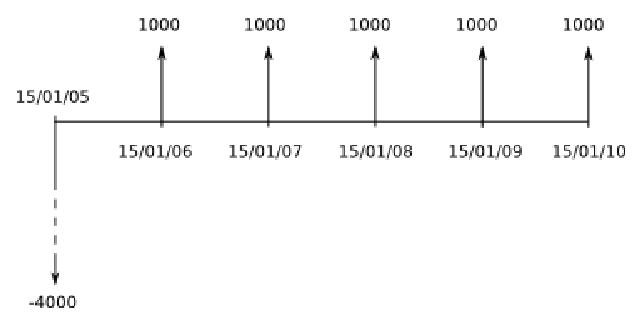
\includegraphics[width=7cm, angle=0]{./images/cashflow.eps}
\caption{Asset cashflow example}
\label{cashflow}
\end{center}
\end{figure}
\FloatBarrier

\emph{Recovery} indicates the expected cash recovered (after taking legal action against 
the borrower) if the borrower defaults at a certain date (see figure \ref{recovery}).

\begin{figure}[!hbt]
\begin{center}
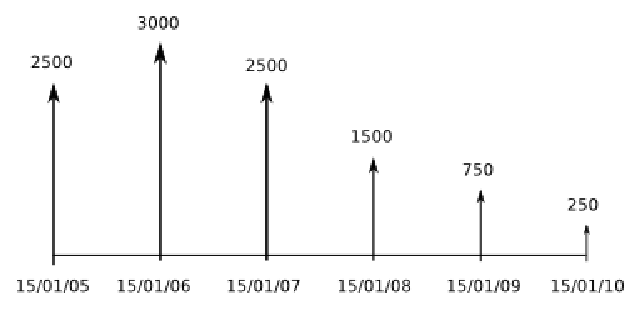
\includegraphics[width=7cm, angle=0]{./images/recovery.eps}
\caption{Asset recovery example}
\label{recovery}
\end{center}
\end{figure}
\FloatBarrier

If a borrower defaults, the loss due to this default is the sum of all remaining
cashflows at default time minus the recovery at default time.

\begin{figure}[!hbt]
\begin{center}
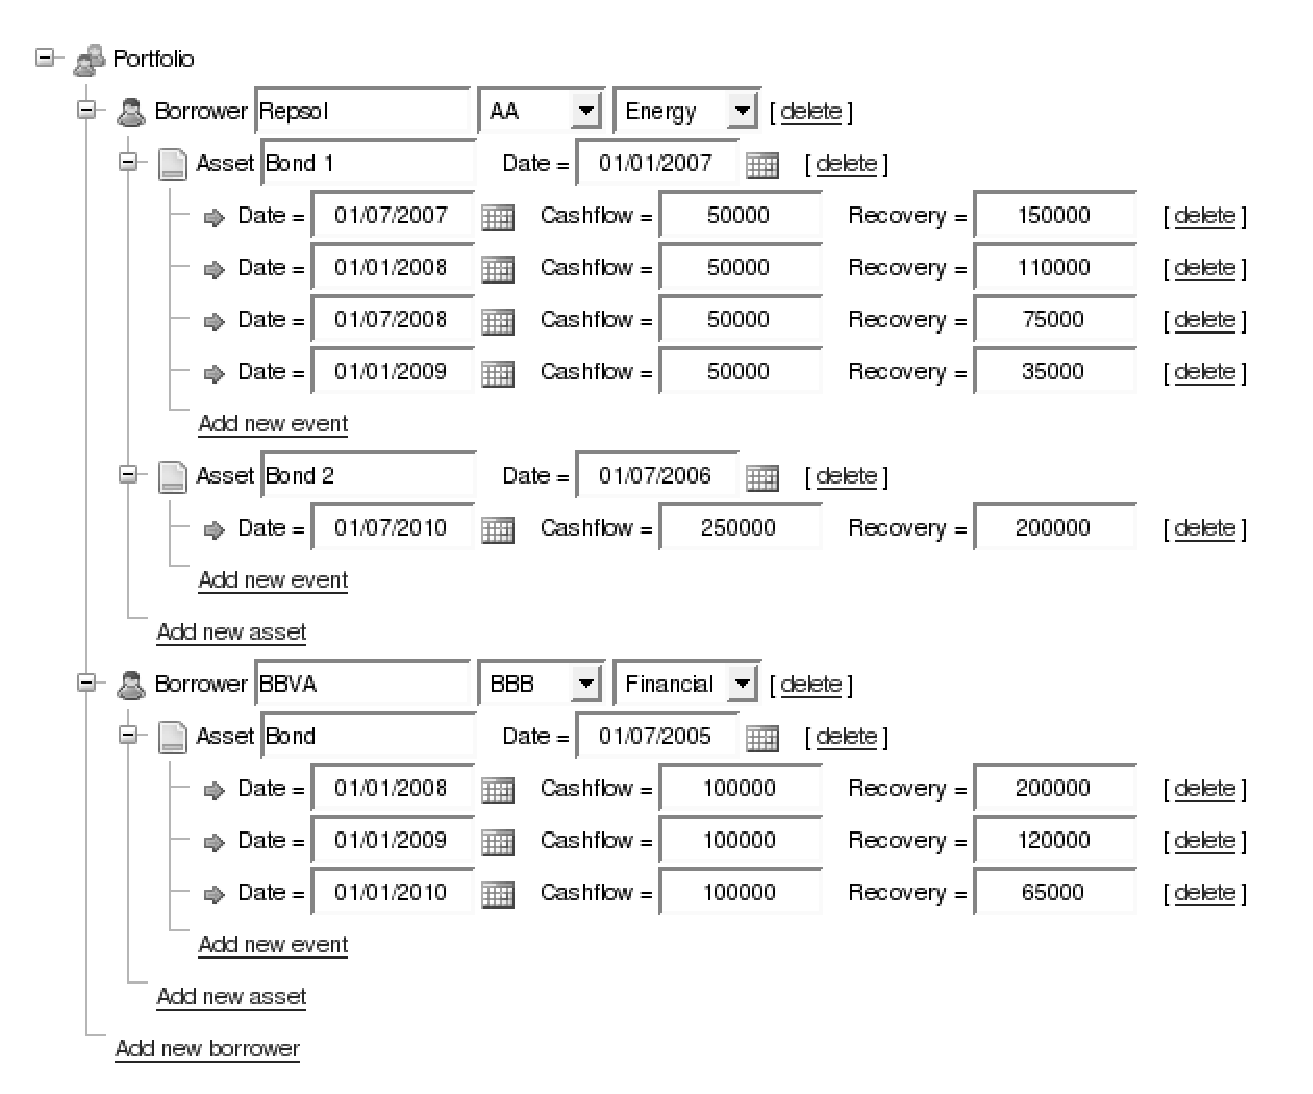
\includegraphics[height=10.5cm, angle=0]{./images/portfolio.eps}
\caption{Portfolio example}
\label{portfolio}
\end{center}
\end{figure}
\FloatBarrier

%===========================================================================
\clearpage
\section{Resolution}

This section explains how CCruncher computes the credit risk of a portfolio.

\begin{figure}[!hb]
\begin{center}
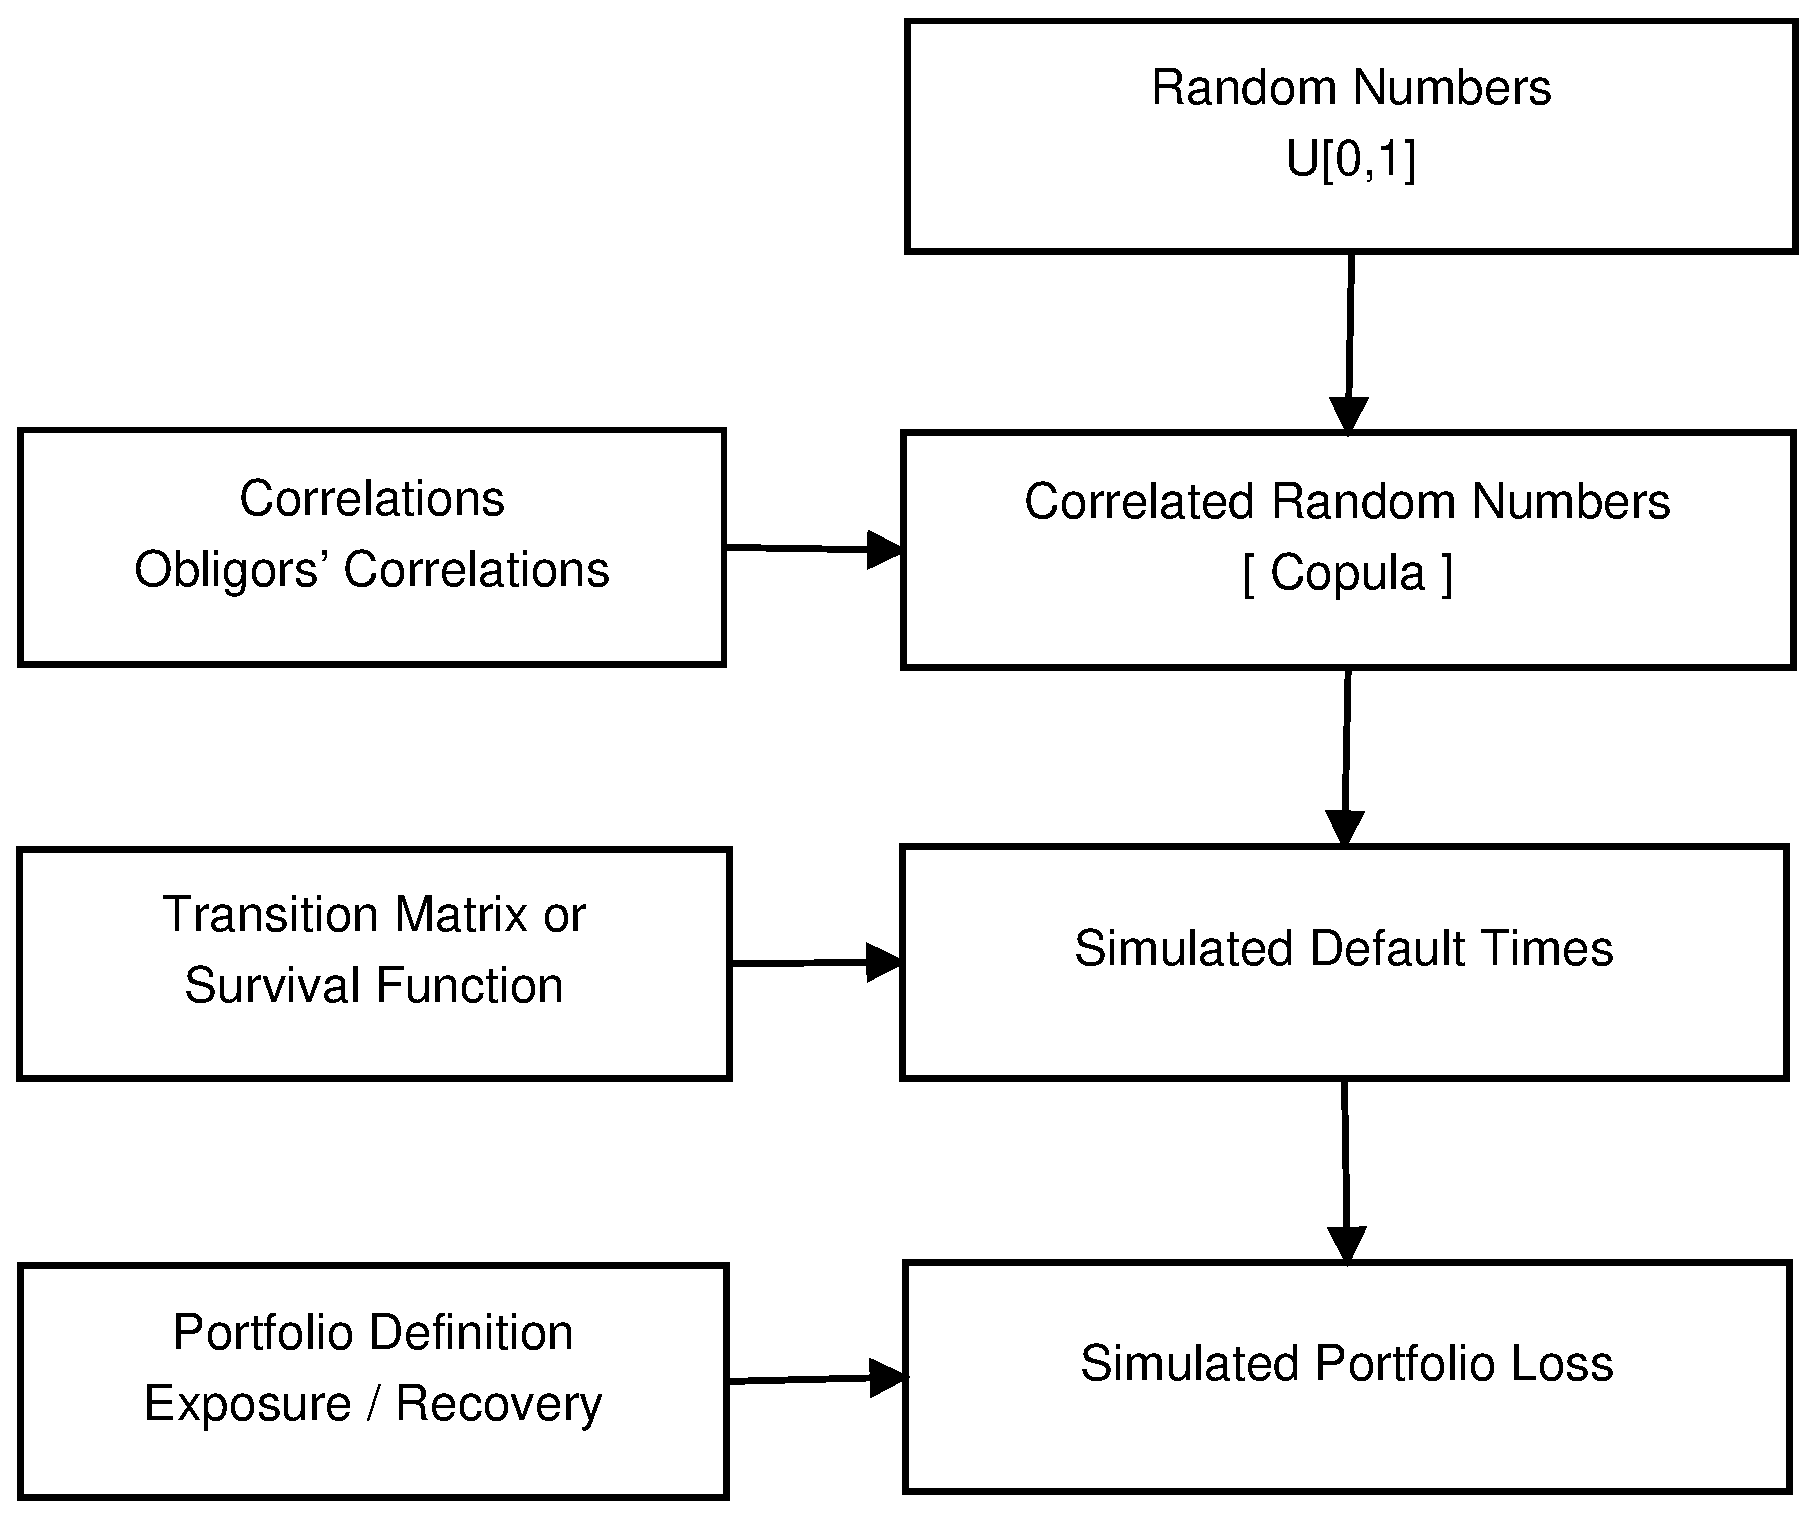
\includegraphics[width=10cm,angle=0]{./images/esquema1.eps}
\caption{Monte Carlo simulation schema}
\label{fig:mcschema1}
\end{center}
\end{figure}

%---------------------------------------------------------------------------
\subsection{Borrowers correlation matrix}
\label{tcorrel}
We need to translate from default correlations between sectors to default 
correlations between borrowers. Let us suppose that we have $n$ borrowers and $m$ 
sectors. Each borrower belongs to a sector. Correlations between sectors are 
known (see \ref{sectors}):

\begin{center}
\begin{tabular}[]{cc}
\begin{tabular}[]{c|ccc}
             & $Sector_1$   & $\dots$  & $Sector_{m}$ \cr
\hline
$Sector_1$   & $\rho_{1,1}$ & $\dots$  & $\rho_{1,m}$ \cr
$\vdots$     & $\vdots$     & $\ddots$ & $\vdots$     \cr
$Sector_{m}$ & $\rho_{1,m}$ & $\dots$  & $\rho_{m,m}$ \cr
\end{tabular}
&
\qquad $\rho_{i,j} = Corr(Sector_i, Sector_j)$
\end{tabular}
\end{center}

We sort the borrowers so that we find those of sector $1$ at the beginning and
those of sector $m$ at the end. Then we create the borrowers correlation matrix 
taking as correlation between two borrowers the correlation between their sectors
(see figure \ref{borrowercorrel}).

\begin{figure}[!hb]
\begin{displaymath}
\begin{array}{c}
\Sigma=
\left(
\begin{array}{ccccccccccc}
1           & \dots    & \rho_{1,1}  &          & \rho_{1,k}  & \dots   & \rho_{1,k}  &         & \rho_{1,m}  & \dots      & \rho_{1,m}  \cr
\vdots      & \ddots   & \vdots      &          & \vdots      &         & \vdots      &         & \vdots      &            & \vdots      \cr
\rho_{1,1}  & \dots    & 1           &          & \rho_{1,k}  & \dots   & \rho_{1,k}  &         & \rho_{1,m}  & \dots      & \rho_{1,m}  \cr

            &          &             & \ddots   &             &         &             &         &             &            &             \cr

\rho_{1,k}  & \dots    & \rho_{1,k}  &          & 1           & \dots   & \rho_{k,k}  &         & \rho_{k,m}  & \dots      & \rho_{k,m}  \cr
\vdots      & \ddots   & \vdots      &          & \vdots      & \ddots  & \vdots      &         & \vdots      &            & \vdots      \cr
\rho_{1,k}  & \dots    & \rho_{1, }  &          & \rho_{k,k}  & \dots   & 1           &         & \rho_{k,m}  & \dots      & \rho_{k,m}  \cr

            &          &             &          &             &         &             & \ddots  &             &            &             \cr

\rho_{1,m}  & \dots    & \rho_{1,m}  &          & \rho_{k,m}  & \dots   & \rho_{k,m}  &         & 1           & \dots      & \rho_{m,m}  \cr
\vdots      & \ddots   & \vdots      &          & \vdots      & \ddots  & \vdots      &         & \vdots      & \ddots     & \vdots      \cr
\rho_{1,m}  & \dots    & \rho_{1,m}  &          & \rho_{k,m}  & \dots   & \rho_{k,m}  &         & \rho_{m,m}  & \dots      & 1           \end{array}
\right)
\end{array}
\end{displaymath}
\caption{Borrowers correlation matrix}
\label{borrowercorrel}
\end{figure}

Observe that this is a correlation matrix (symmetric, $|\rho_{i,j}| \leq 1$, 
$|\rho_{i,i}| = 1$) composed by blocks. This matrix will be decomposed using 
the Cholesky algorithm, so it must be definite positive.

%---------------------------------------------------------------------------
\subsection{Monte Carlo simulation}
\label{mcsim}
Monte Carlo methods are a class of computational algorithms for 
simulating the behavior of various physical and mathematical systems. 
Each simulation consists of computing a random default time for each borrower and
then calculate the loss of the portfolio. We need that default times fulfill two 
conditions: the borrower's survival functions and the borrower's correlation matrix. 
This is achieved by simulating a copula. 

%...........................................................................
\subsubsection{Random numbers generation}
A copula \cite{copu:pitfalls} \cite{copu:wang} is a multivariate random variable 
where each component is a uniform $U[0,1]$. Each simulation requires a set of 
random numbers between $[0, 1]$ and correlated by the borrowers' correlation 
matrix, $\Sigma$ (see figure \ref{borrowercorrel}).

\begin{displaymath}
\begin{array}{ccc}
\begin{array}{|c|c|c|c|}
u_{11} & u_{12} & \dots  & u_{1n} \cr
u_{21} & u_{22} & \dots  & u_{2n} \cr
\vdots & \vdots & \vdots & \vdots \cr
u_{k1} & u_{k2} & \dots  & u_{kn} \cr
\end{array}
&
\qquad
&
\begin{array}{c}
n \textrm{ number of borrowers} \cr
k \textrm{ number of simulations} \cr
u_{.i} \sim U[0,1] \cr
Corr(u_{.i}, u_{.j}) = \Sigma_{ij} \cr
\end{array}
\end{array}
\end{displaymath}

There are implemented two copula generators, the gaussian and the t-Student
copulas. Apendices \ref{ap:gaussiancopu} and \ref{ap:tstudentcopu} describes the 
algorithms used to generate them.
\newline

Exists evidences \cite{copu:selecting} in favor of the t-Student copula. 
In comparison with the t-Student copula, gaussian copula underestimates the probability 
of joint extreme downward movements. Moreover gaussian copula is too optimistic on 
diversification benefits.

%...........................................................................
\subsubsection{Default times simulation}
\label{sec:deftimessim}
Given the borrower $k$ and the random number $u_k \in [0,1]$ (generated using a 
copula in the previous step) we simulate the default time considering the 
inverse of the borrower survival function at $u_k$ \cite{ref:cred_risk}. 
Figure \ref{simttd} shows this in a graphic manner.

\begin{figure}[!hbt]
\begin{center}
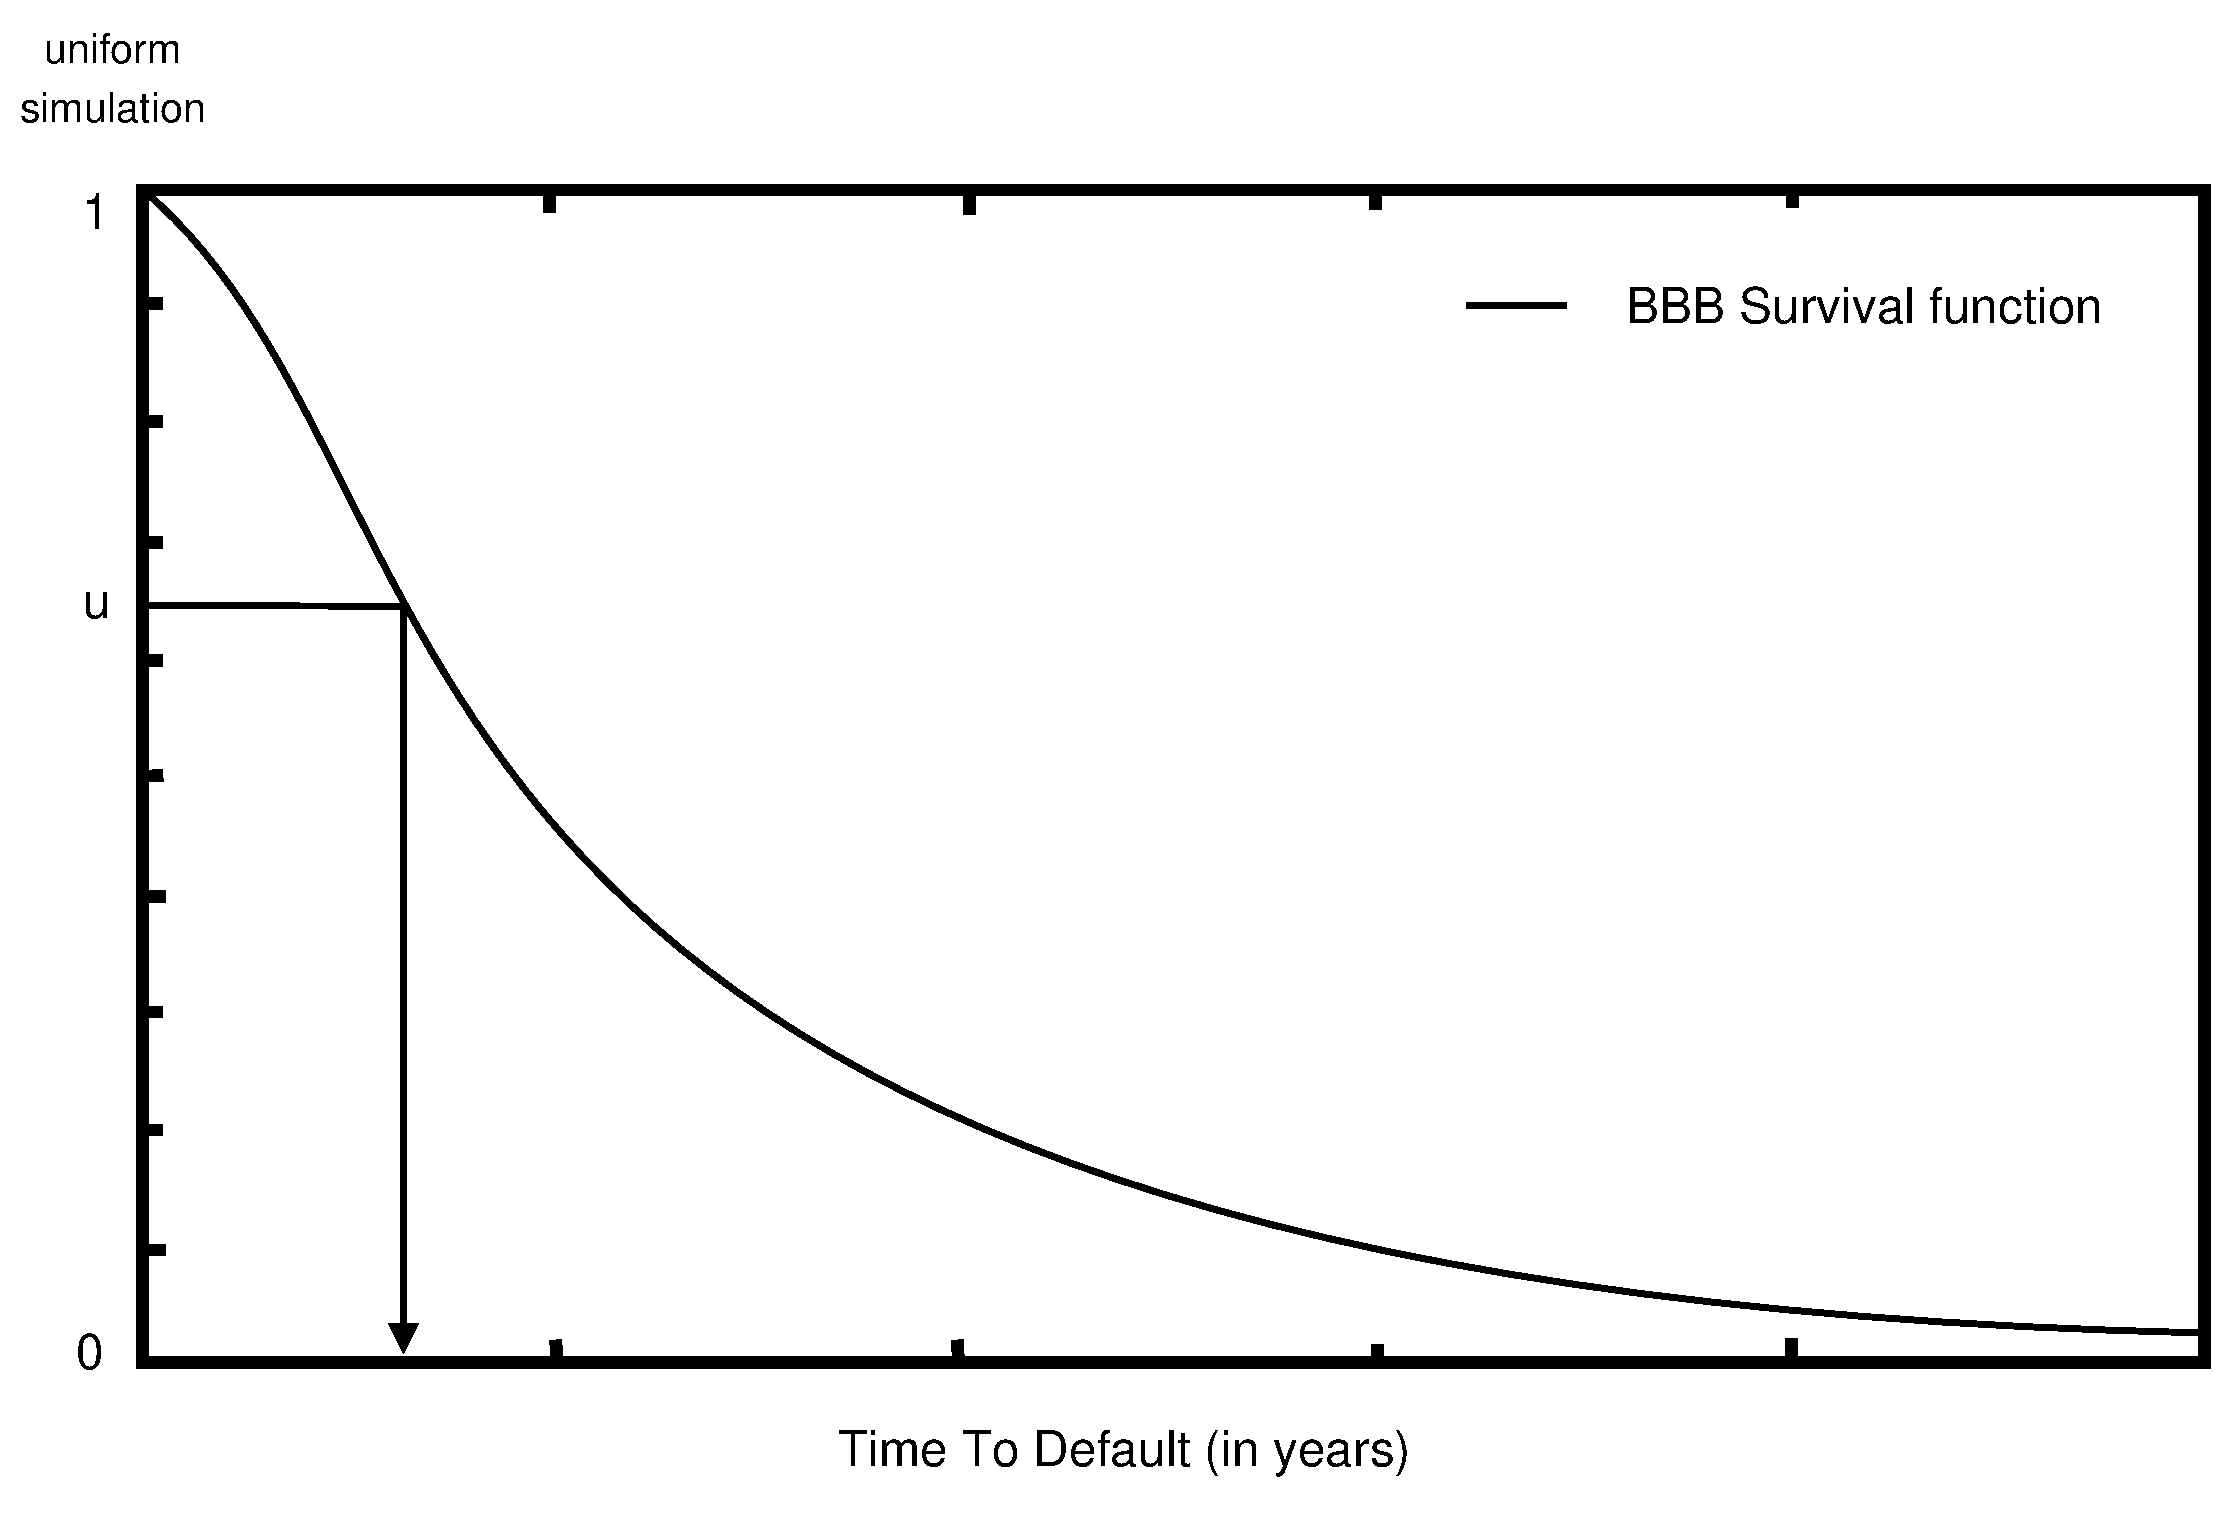
\includegraphics[width=10cm,angle=0]{./images/simttd.eps}
\caption{Default time generation with initial rating $BBB$}
\label{simttd}
\end{center}
\end{figure}
\FloatBarrier

%...........................................................................
\subsubsection{Portfolio loss evaluation}
\label{sec:portfolioloss}
At this point, given any borrower, we have a simulated default time. The loss
caused by this borrower is the sum of all remaining cashflows at default time 
minus the recovery at default default time. To obtain the simulated 
value of the portfolio loss we sum all losses and we keep this value 
in a list. Afterwards we will use this list to compute risk.
\newline

%TODO: add a graphic

We consider the recovery at default time as the closest asset recovery by right.
Figure \ref{recoverymapping} shows distinct default times and its recovery 
values (bolded lines) using recoveries defined in figure \ref{recovery} 
(grayed lines).

\begin{figure}[!hbtp]
\begin{center}
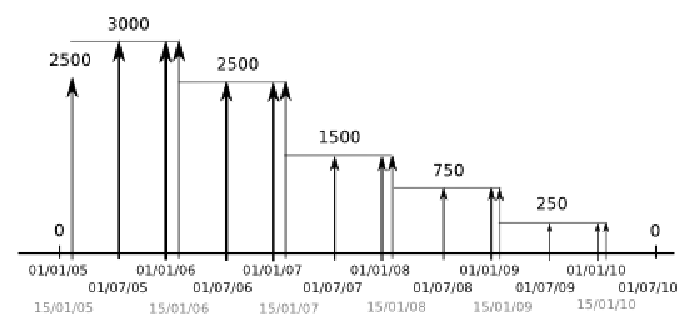
\includegraphics[width=12cm, angle=0]{./images/recoverymapping.eps}
\caption{Asset recoveries in distinct default times}
\label{recoverymapping}
\end{center}
\end{figure}
\FloatBarrier

%---------------------------------------------------------------------------
\subsection{Risk computation}
After $N$ simulations (eg. $20000$, $500000$ or more) we have a list
of numbers, ${x_1, ..., x_N}$, where each number represents a simulated portfolio 
loss. The more values, the more accuracy in the results. All risk statistics (eg. 
Expected Loss) have an error margin that will be estimated. CCruncher uses 
\emph{R package}\footnote{http://www.r-project.org} to perform the statistical
computations described below.
\newline

First of all we can approximate the probability distribution of the portfolio 
loss creating an histogram with the simulated values.

\begin{figure}[!hbt]
\begin{center}
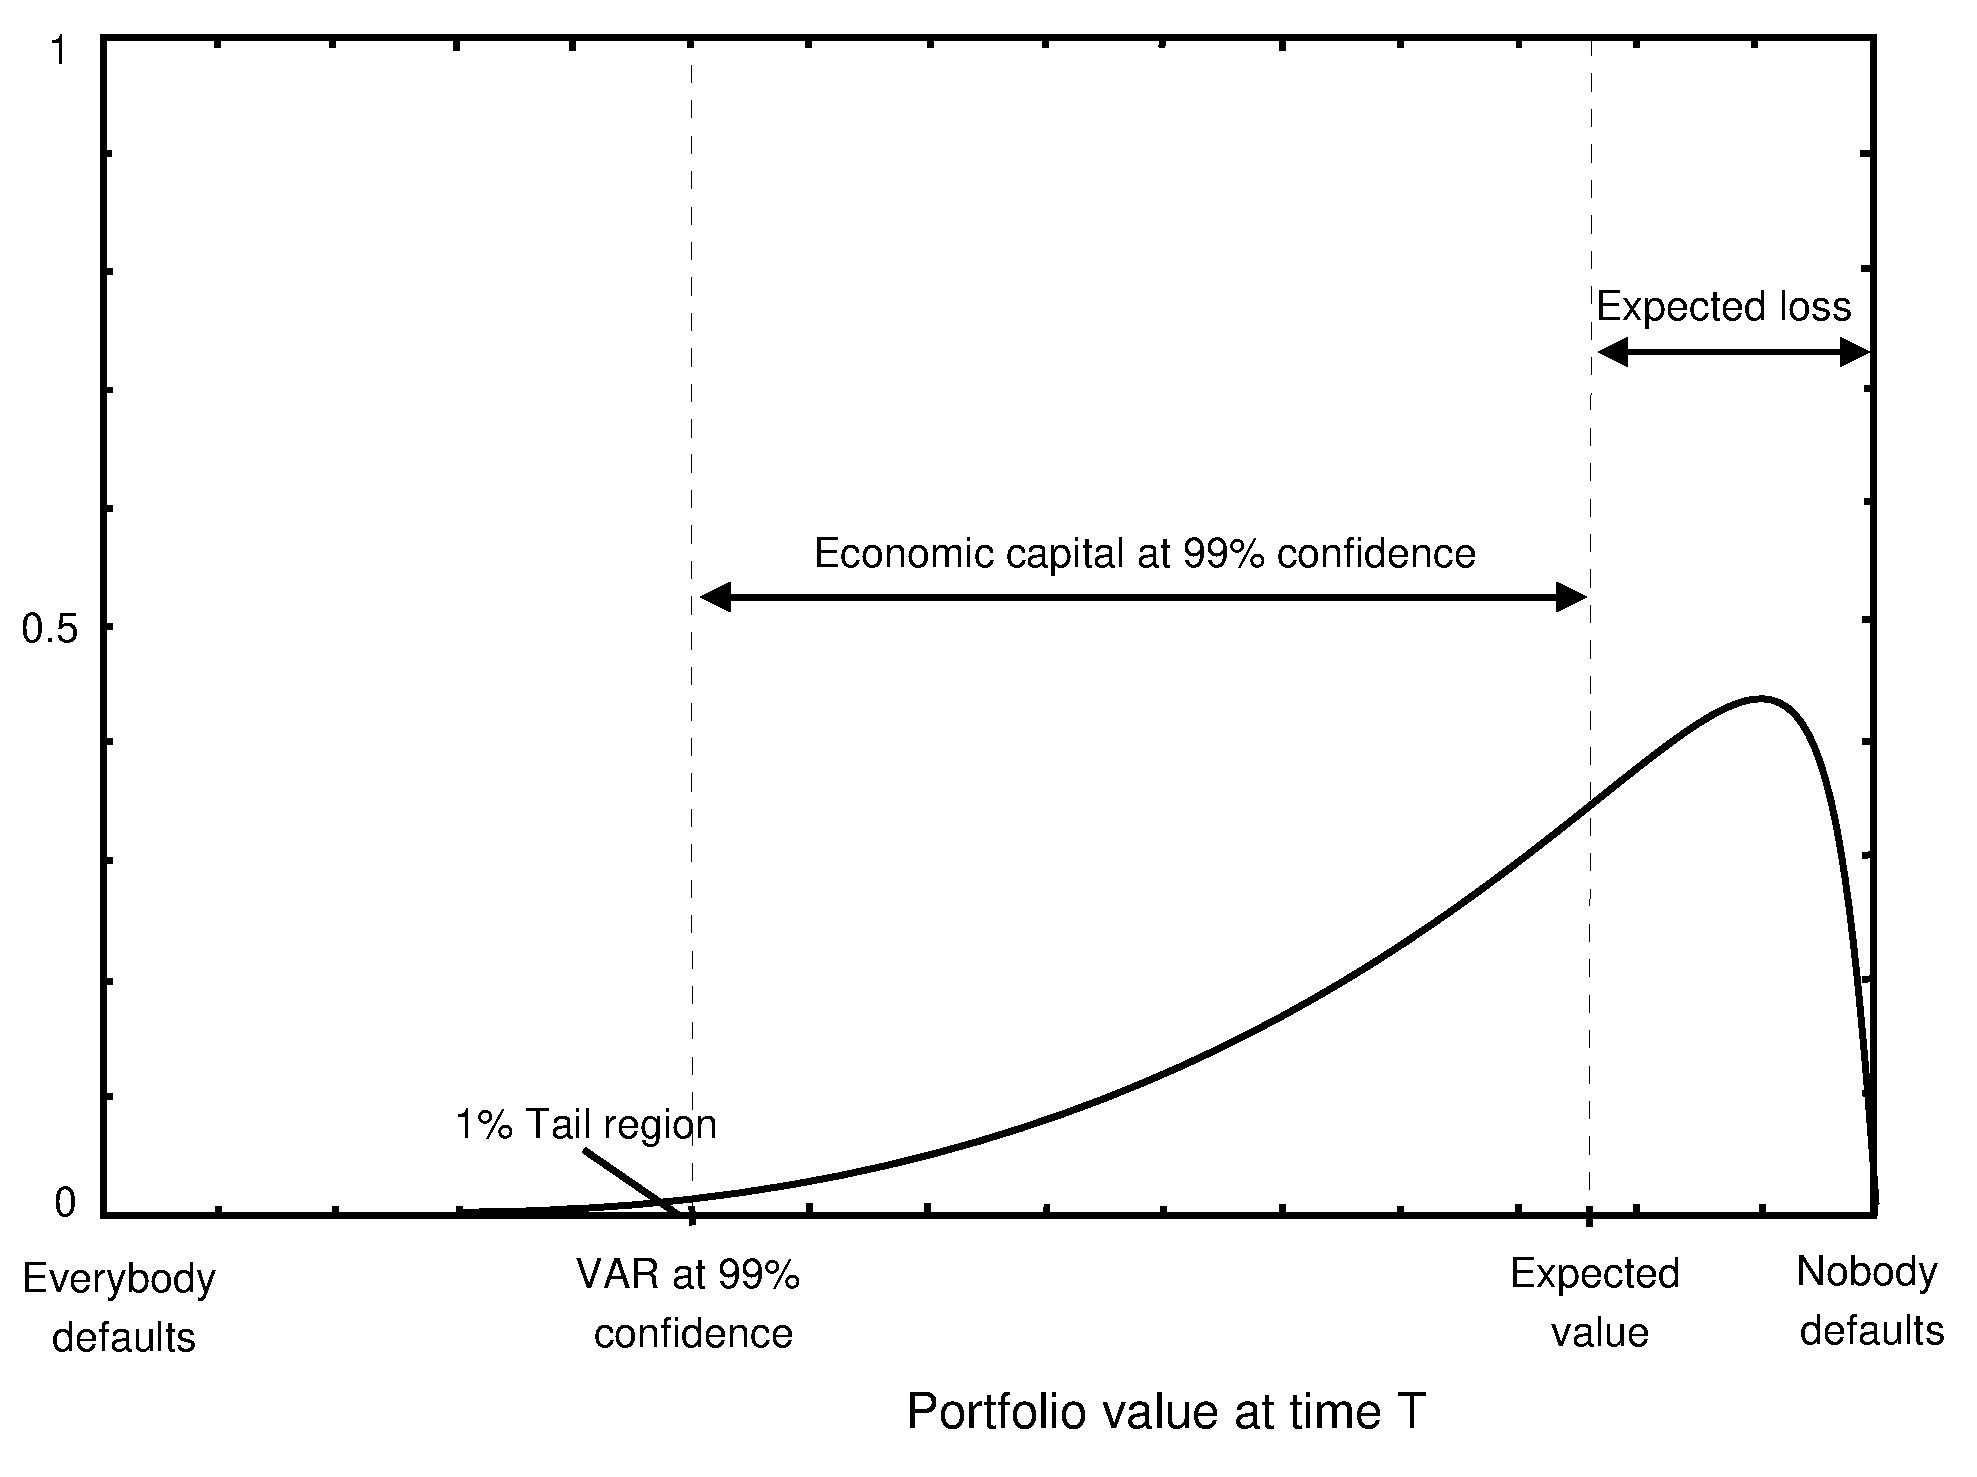
\includegraphics[height=7cm, angle=0]{./images/creditvar.eps}
\caption{Portfolio loss at time $T$}
\label{creditvar}
\end{center}
\end{figure}
\FloatBarrier

%...........................................................................
\subsubsection{Expected Loss}
Expected Loss is the probability distribution mean of the portfolio loss.
Central Limit Theorem \cite{stats:schaum} grants that:

\begin{displaymath}
\mu = \widehat{\mu} \pm \phi^{-1}\left(\frac{1-\alpha}{2}\right) \cdot \frac{\widehat{\sigma}}{\sqrt{N}}
\end{displaymath}
where $\alpha$ is the error confidence level, $\phi^{-1}$ the N(0,1) inverse 
cumulative distribution function and $\widehat{\mu}$ and $\widehat{\sigma}$ are 
the mean and stddev estimators:

\begin{displaymath}
\widehat{\mu} = \frac{1}{N} \sum_{i=1}^{N} x_i
\end{displaymath}

\begin{displaymath}
\widehat{\sigma} =
\sqrt{\frac{1}{N-1} \sum_{i=1}^{N} \left( x_i - \widehat{\mu} \right)^2} =
\sqrt{\frac{1}{N-1} \left( \sum_{i=1}^{N} x_i^2 - \frac{\left(\sum_{i=1}^{N} x_i \right)^2}{N} \right)}
\end{displaymath}

%...........................................................................
\subsubsection{Portfolio Loss Standard Deviation}
Another usual risk statistic is the standard deviation of the portfolio loss.
Central Limit Theorem \cite{stats:schaum} grants that:

\begin{displaymath}
\sigma = \widehat{\sigma} \pm \phi^{-1}\left(\frac{1-\alpha}{2}\right) \cdot \frac{\widehat{\sigma}}{\sqrt{2N}}
\end{displaymath}

where $\alpha$ is the error confidence level, $\phi^{-1}$ the N(0,1) inverse 
cumulative distribution function and $\widehat{\sigma}$ is the stddev estimator
defined previously.

%...........................................................................
\subsubsection{Value At Risk}
Value at Risk \cite{var:jorion} is the most used risk value. We call it 
$VAR_{\beta}$ where $\beta$ is the VAR confidence level (eg. VAR at $95\%$).
VAR is another form to say quantile. Then
$VAR_{\beta} = q_{\beta} = \textrm{inf}\{x | F(x) \geq \beta \}$. 

\begin{displaymath}
VAR_{\beta} = \widehat{q_{\beta}} \pm \phi^{-1}\left(\frac{1-\alpha}{2}\right) \cdot \textrm{stderr}(q_{\beta})
\end{displaymath}

where $\alpha$ is the error confidence level, $\beta$ is the VAR confidence 
level, $\phi^{-1}$ the N(0,1) inverse cumulative distribution function, 
$\widehat{q_{\beta}}$ is the quantile estimator, and $\textrm{stderr}(q_{\beta})$
is the estimation of the standard error.

\begin{displaymath}
\widehat{q_{\beta}} = x_{k:N}
\end{displaymath}
where,
\begin{itemize}
\item $k$ fulfills $\frac{k}{N} \leq \beta < \frac{k+1}{N}$
\item $x_{k:N}$ is the $k$-th element of ascendent sorted values
\end{itemize}

We determine $\textrm{stderr}(q_{\beta})$ using Maritz-Jarret method described
in \cite{quant:algor}.

\begin{eqnarray}
M   & = & [N \beta + 0.5] \nonumber \\
a   & = & M - 1 \nonumber \\
b   & = & N - M \nonumber \\
W_i & = & B(a,b,\frac{i+1}{N}) - B(a,b,\frac{i}{N}) \nonumber \\
C_k & = & \sum_{i=1}^{N} W_i \cdot x_i \nonumber
\end{eqnarray}

where $[x]$ is the integer part of $x$ and $B(a,b,x)$ is the incomplete beta 
function:

\begin{displaymath}
B(a,b,x)=\frac{\Gamma(a+b)}{\Gamma(a)\Gamma(b)}\int_0^x t^{a-1} (1-t)^{b-1} dt
\end{displaymath}

Then,
\begin{displaymath}
\textrm{stderr}(q_{\beta}) = \sqrt{C_2 - C_1^2}
\end{displaymath}

%...........................................................................
\subsubsection{Expected Shortfall}
VAR is not a distance because it does not fulfill the sub-additive property 
\cite{var:varbad}, $VAR(A+B) \nleq VAR(A)+VAR(B)$. Expected Shortfall is a 
consistent risk measure \cite{var:eshortfall} similar to VAR. It can be described
as the average of the $\beta\%$ worst losses.

\begin{displaymath}
ES_{\beta} = \widehat{ES_{\beta}} \pm \phi^{-1}\left(\frac{1-\alpha}{2}\right) \cdot \textrm{stderr}(ES_{\beta})
\end{displaymath}

where $\alpha$ is the error confidence level, $\beta$ is the ES confidence 
level, $\phi^{-1}$ the N(0,1) inverse cumulative distribution function, 
$\widehat{ES_{\beta}}$ is the ES estimator and $\textrm{stderr}(ES_{\beta})$
is the estimation of the standard error.
\newline

We select the simulation portfolio loss values ($x_1, ..., x_N$) that are bigger 
than $VAR_{\beta}$.

\begin{displaymath}
y_1, y_2, y_3, \cdots, y_K \qquad \textrm{where} \quad y_i > VAR_{\beta}
\end{displaymath}

Then,

\begin{displaymath}
\widehat{ES_{\beta}} = \frac{1}{K} \sum_{i=1}^{K} y_i
\end{displaymath}

\begin{displaymath}
\textrm{stderr}(ES_{\beta}) =
\frac{\sqrt{\frac{1}{K-1} \sum_{i=1}^{K} \left( y_i - \widehat{ES_{\beta}} \right)^2}}{\sqrt{K}} =
\frac{\sqrt{\frac{1}{K-1} \left( \sum_{i=1}^{K} y_i^2 - \frac{\left(\sum_{i=1}^{K} y_i \right)^2}{K} \right)}}{\sqrt{K}}
\end{displaymath}

%...........................................................................
\subsubsection{Economic Capital}
We can compute the Economic Capital at confidence level $\beta$ as:

\begin{displaymath}
\textrm{Economic Capital} = VAR_{\beta} - \textrm{Expected Loss}
\end{displaymath}

%...........................................................................

\begin{figure}[p]
\begin{center}
\includegraphics[width=12cm,angle=0]{./images/report.eps}
\caption{CCruncher results}
\label{report}
\end{center}
\end{figure}


%===========================================================================
\clearpage
\section{Other considerations}
CCruncher takes into consideration other concepts that have not been exposed 
up to this moment with the purpose of simplifying the content.

%---------------------------------------------------------------------------
\subsection{Risk aggregation}
CCruncher simulates the whole portfolio loss at time $T$. It also allows (in 
the same execution) the simulation of subportfolios by defining one or more 
aggregators. Consequently you can determine which are the borrowers (or products 
or branches or regions or assets, etc.) that increase the risk of your portfolio. 
Every subportfolio has its own list of simulated values that can be processed to 
obtain the risk indicators for this subportfolio.

%---------------------------------------------------------------------------
\subsection{Yield curve}
CCruncher can consider that money value decreases along the time following a fixed 
curve (eg. yield curve). CCruncher allows the input of the yield curve and and takes
it into account in all its computations. The coeficient that determines the money 
value decreases along the time is given by the compound interest formula:

\begin{displaymath}
\Upsilon(r, t_0,t_1) = (1+r)^{(t_1-t_0)}
\end{displaymath}

%---------------------------------------------------------------------------
\subsection{Antithetic technique}
The random number generation using a copula is time expensive. Gaussian and 
t-Student copula are symmetric, that means that $(u_1, u_2, \cdots, u_n)$ is 
equiprobable to $(1-u_1, 1-u_2, \cdots, 1-u_n)$. In CCruncher's antithetic mode, 
each copula generation is used $2$ times, $(u_1, u_2, \cdots, u_n)$ and 
$(1-u_1, 1-u_2, \cdots, 1-u_n)$, reducing to the half the number of generated
copulas.

%---------------------------------------------------------------------------
\subsection{Parallel computing}
Monte Carlo problems are embarrassingly parallel problems.
In the jargon of parallel computing, an embarrassingly parallel workload 
(or embarrassingly parallel problem) is one for which no particular effort 
is needed to segment the problem into a very large number of parallel tasks, 
and there is no essential dependency (or communication) between those parallel 
tasks.
\newline

In CCruncher the master sends the RNG seed to each slave 
($seed_i = seed + i \cdot 30001$) and waits for results (the simulated values of
the portfolio loss) from slaves that store them in a file. When one of the two stop 
criteria is achieved (maximum execution time exceded or maximum number of 
simulations reached) the master sends a stop signal to the slaves and leaves.


%===========================================================================
\section{Numerical example}

Lets go to compute the credit risk at $T=30$ years for the following portfolio.

\begin{table}[!hb]
\begin{center}
\begin{tabular}[]{c|l|c|c|c|l}
Id  & Borrower name        & Rating & Sector         & Recovery & Assets     \cr
\hline
B1  & Future Skyline       & AA     & Construction   & 80\%     & A1         \cr
B2  & Ramses builds        & BBB    & Construction   & 75\%     & A2, A3     \cr
B3  & Gramdateresi         & AA     & Consumer goods & 60\%     & A4         \cr
B4  & Tantor Pinori        & BB     & Consumer goods & 90\%     & A5, A6, A7 \cr
B5  & White \& Rebolan     & B      & Services       & 30\%     & A8         \cr
B6  & Adign Consulting     & BBB    & Services       & 60\%     & A9         \cr
B7  & Advanced Engineering & AAA    & Services       & 50\%     & A10        \cr
B8  & Sigmacle Research    & CCC    & Services       & 60\%     & A11        \cr
B9  & Loglament Asia       & AA     & Services       & 50\%     & A12        \cr
\end{tabular}
\caption{Portfolio composition}
\label{example.portfolio}
\end{center}
\end{table}

The following table list the assets events in months from current date.

\begin{table}[!hb]
\begin{center}
\begin{tabular}[]{c|c|c|c|c|c|c|c|c|c|c|c|c}
Month & A1   & A2   & A3   & A4   & A5   & A6   & A7   & A8   & A9   & A10  & A11  & A12   \cr
\hline
6     & 10 \$&      &      &      &100 \$&      &      &      &      &      &      & 70 \$ \cr
12    &      & 50 \$&      &      &      & 20 \$& 80 \$&      & 20 \$&      &      &       \cr
36    &      &      &      &      &      &      &      &      &      &      & 30 \$&       \cr
60    &      & 30 \$&      &      & 10 \$&      & 20 \$& 80 \$&      &      &      &       \cr
90    &      &      &      &      &      & 30 \$&      &      &      &      &      &       \cr
120   & 15 \$&      & 40 \$&      & 30 \$&      &      &      &      &      &      &       \cr
180   &      &      &      &      & 40 \$& 70 \$&      &      &      &      &      &       \cr
216   &      & 10 \$&      &      & 50 \$&      &      &      &      &      &      & 80 \$ \cr
240   &      &      &      &100 \$&      &      &      &      &      &      &      &       \cr
312   &100 \$&      & 40 \$&      & 70 \$&      &      &      & 70 \$&      &      &       \cr
360   &      &      &      &      &      & 15 \$&      &      &      &      & 40 \$&       \cr
384   & 90 \$&      &      &      & 90 \$&      &      &      &      &100 \$& 90 \$&             
\end{tabular}
\caption{Assets events}
\label{example.assets}
\end{center}
\end{table}

In this example we supose that we don't dispose of survival functions but we have the transition
matrix $T_1$ (extracted from \cite{CreditMetrics:Tech_Doc}).

\begin{table}[!hb]
\begin{center}
\begin{tabular}[]{l|rrrrrrrr}
        &      AAA &       AA &        A &      BBB &       BB &        B &      CCC &  Default \cr
\hline
AAA     &  $90.81$ &   $8.33$ &   $0.68$ &   $0.06$ &   $0.12$ &   $0.00$ &   $0.00$ &   $0.00$ \cr
 AA     &   $0.70$ &  $90.65$ &   $7.79$ &   $0.64$ &   $0.06$ &   $0.14$ &   $0.02$ &   $0.00$ \cr
  A     &   $0.09$ &   $2.27$ &  $91.05$ &   $5.52$ &   $0.74$ &   $0.26$ &   $0.01$ &   $0.06$ \cr
BBB     &   $0.02$ &   $0.33$ &   $5.95$ &  $86.93$ &   $5.30$ &   $1.17$ &   $0.12$ &   $0.18$ \cr
 BB     &   $0.03$ &   $0.14$ &   $0.67$ &   $7.73$ &  $80.53$ &   $8.84$ &   $1.00$ &   $1.06$ \cr
  B     &   $0.00$ &   $0.11$ &   $0.24$ &   $0.43$ &   $6.48$ &  $83.46$ &   $4.07$ &   $5.21$ \cr
CCC     &   $0.22$ &   $0.00$ &   $0.22$ &   $1.30$ &   $2.38$ &  $11.24$ &  $64.86$ &  $19.78$ \cr
Default &   $0.00$ &   $0.00$ &   $0.00$ &   $0.00$ &   $0.00$ &   $0.00$ &   $0.00$ & $100.00$
\end{tabular}
\caption{$1$-year transition matrix}
\label{example.tmatrix}
\end{center}
\end{table}

The default times sectorial correlations are:

\begin{table}[!hb]
\begin{center}
\begin{tabular}[]{c|ccc}
               & Construction & Consumer goods & Services \cr
\hline
Construction   &    $0.50$    &     $0.20$     &   $0.30$ \cr
Consumer goods &    $0.20$    &     $0.60$     &   $0.34$ \cr
Services       &    $0.30$    &     $0.34$     &   $0.40$ 
\end{tabular}
\caption{Sector correlation matrix}
\label{example.scorrels}
\end{center}
\end{table}

%---------------------------------------------------------------------------
\subsection{Obtaining the survival functions}

We use appendix \ref{ap:tmatrix} to compute the survivals functions 
with a time resolution of $1$ month. We scale the transition matrix 
to $1$ month doing $T_{\frac{1}{12}} = T_{1}^{\frac{1}{12}}$. Caution, 
do calculations using absolute values, not percentages. $1$-month 
transition matrix, $T_{\frac{1}{12}}$:

{\small
\begin{displaymath}
%T_{\frac{1}{12}} = 
\left( 
\begin{array}{cccccccc}
    99.1972  &   0.7588  &   0.0320  &   0.0020  &   0.0112  &  -0.0011  &  -0.0001  &   0.0000  \cr
     0.0635  &  99.1745  &   0.7083  &   0.0392  &   0.0015  &   0.0120  &   0.0018  &  -0.0007  \cr
     0.0074  &   0.2057  &  99.1980  &   0.5102  &   0.0557  &   0.0189  &  -0.0001  &   0.0042  \cr
     0.0015  &   0.0239  &   0.5507  &  98.8021  &   0.5164  &   0.0871  &   0.0077  &   0.0107  \cr
     0.0027  &   0.0113  &   0.0396  &   0.7581  &  98.1558  &   0.8774  &   0.0889  &   0.0664  \cr
    -0.0007  &   0.0098  &   0.0196  &   0.0111  &   0.6447  &  98.4443  &   0.4463  &   0.4249  \cr
     0.0233  &  -0.0023  &   0.0170  &   0.1287  &   0.2166  &   1.2298  &  96.4213  &   1.9657  \cr
     0.0000  &   0.0000  &   0.0000  &   0.0000  &   0.0000  &   0.0000  &   0.0000  & 100.0000 
\end{array}
\right)
\end{displaymath}
}

Note negative values in the computed $1$-month transition matrix. Something wrong happens 
because transition matrix values are probabilities. The cause is that the original matrix 
$T_1$ is not a regular Markov matrix. In this cases CreditCruncher replace negative 
values by $0$.
\newline

One time we dispose $1$-month transition matrix, we compute the survivals
values at month $1$ doing ($d$ subindex means default column):

\begin{displaymath}
S(.,1 \textrm{ month}) = \vec{1} - (T_{1/12})_{.d} = 
\left( 
\begin{array}{c}
 100 \cr
 100 \cr
 100 \cr
 100 \cr
 100 \cr
 100 \cr
 100
\end{array}
\right)
 - 
\left( 
\begin{array}{c}
 0.0000 \cr
 0.0000 \cr
 0.0042 \cr
 0.0107 \cr
 0.0664 \cr
 0.4249 \cr
 1.9657
\end{array}
\right)
=
\left( 
\begin{array}{c}
 100.000 \cr
 100.000 \cr
  99.996 \cr
  99.989 \cr
  99.934 \cr
  99.975 \cr
  98.034 
\end{array}
\right)
\end{displaymath}

We compute the survivals values at month $2$ doing:

\begin{displaymath}
S(.,2 \textrm{ months}) = \vec{1} - (T_{1/12}^2)_{.d} = 
\left( 
\begin{array}{c}
 100 \cr
 100 \cr
 100 \cr
 100 \cr
 100 \cr
 100 \cr
 100
\end{array}
\right)
 - 
\left( 
\begin{array}{c}
 0.0000 \cr
 0.0000 \cr
 0.0084 \cr
 0.0221 \cr
 0.1372 \cr
 0.8524 \cr
 3.8664
\end{array}
\right)
=
\left( 
\begin{array}{c}
 100.000 \cr
 100.000 \cr
  99.992 \cr
  99.978 \cr
  99.863 \cr
  99.148 \cr
  96.134 
\end{array}
\right)
\end{displaymath}

We compute the survivals values at month $3$ doing:

\begin{displaymath}
S(.,3 \textrm{ months}) = \vec{1} - (T_{1/12}^3)_{.d} = 
\left( 
\begin{array}{c}
 100 \cr
 100 \cr
 100 \cr
 100 \cr
 100 \cr
 100 \cr
 100
\end{array}
\right)
 - 
\left( 
\begin{array}{c}
 0.0000 \cr
 0.0000 \cr
 0.0129 \cr
 0.0342 \cr
 0.2122 \cr
 1.2821 \cr
 5.7045
\end{array}
\right)
=
\left( 
\begin{array}{c}
 100.000 \cr
 100.000 \cr
  99.987 \cr
  99.966 \cr
  99.788 \cr
  98.718 \cr
  94.296 
\end{array}
\right)
\end{displaymath}

If we repeat the same procedure for the $36$ month we obtain the survival
function exposed at table \ref{example.survivals}.

\clearpage 

\begin{table}[!hb]
\begin{center}
{\small
\begin{tabular}[]{c|rrrrrrrr}
Month &  AAA   &  AA    &   A    &  BBB   &  BB    &   B    &  CCC   \cr
\hline
1  & 100.000 & 100.000 &  99.996 &  99.989 &  99.934 &  99.575 &  98.034 \cr
2  & 100.000 & 100.000 &  99.992 &  99.978 &  99.863 &  99.148 &  96.134 \cr
3  & 100.000 & 100.000 &  99.987 &  99.966 &  99.788 &  98.718 &  94.296 \cr
4  & 100.000 & 100.000 &  99.983 &  99.953 &  99.709 &  98.286 &  92.518 \cr
5  & 100.000 & 100.000 &  99.978 &  99.939 &  99.626 &  97.853 &  90.798 \cr
6  & 100.000 & 100.000 &  99.973 &  99.925 &  99.539 &  97.418 &  89.134 \cr
7  & 100.000 & 100.000 &  99.968 &  99.909 &  99.448 &  96.981 &  87.525 \cr
8  & 100.000 & 100.000 &  99.963 &  99.893 &  99.353 &  96.544 &  85.967 \cr
9  & 100.000 & 100.000 &  99.957 &  99.876 &  99.255 &  96.106 &  84.460 \cr
10 & 100.000 & 100.000 &  99.952 &  99.858 &  99.153 &  95.668 &  83.000 \cr
11 & 100.000 & 100.000 &  99.946 &  99.840 &  99.048 &  95.229 &  81.588 \cr
12 & 100.000 & 100.000 &  99.940 &  99.820 &  98.940 &  94.790 &  80.220 \cr
13 & 100.000 &  99.999 &  99.934 &  99.800 &  98.828 &  94.351 &  78.896 \cr
14 & 100.000 &  99.998 &  99.928 &  99.778 &  98.714 &  93.912 &  77.613 \cr
15 & 100.000 &  99.997 &  99.921 &  99.756 &  98.596 &  93.474 &  76.370 \cr
16 & 100.000 &  99.996 &  99.914 &  99.733 &  98.475 &  93.036 &  75.167 \cr
17 & 100.000 &  99.995 &  99.907 &  99.710 &  98.352 &  92.599 &  74.000 \cr
18 &  99.999 &  99.993 &  99.900 &  99.685 &  98.225 &  92.162 &  72.870 \cr
19 &  99.999 &  99.992 &  99.893 &  99.660 &  98.096 &  91.727 &  71.775 \cr
20 &  99.999 &  99.990 &  99.885 &  99.633 &  97.965 &  91.292 &  70.713 \cr
21 &  99.999 &  99.988 &  99.877 &  99.606 &  97.831 &  90.859 &  69.683 \cr
22 &  99.999 &  99.986 &  99.869 &  99.578 &  97.694 &  90.427 &  68.685 \cr
23 &  99.998 &  99.984 &  99.861 &  99.549 &  97.555 &  89.996 &  67.717 \cr
24 &  99.998 &  99.982 &  99.852 &  99.519 &  97.414 &  89.567 &  66.777 \cr
25 &  99.998 &  99.980 &  99.843 &  99.488 &  97.270 &  89.139 &  65.866 \cr
26 &  99.998 &  99.978 &  99.834 &  99.457 &  97.125 &  88.714 &  64.982 \cr
27 &  99.997 &  99.975 &  99.825 &  99.424 &  96.977 &  88.289 &  64.124 \cr
28 &  99.997 &  99.972 &  99.815 &  99.391 &  96.827 &  87.867 &  63.290 \cr
29 &  99.996 &  99.970 &  99.805 &  99.357 &  96.675 &  87.446 &  62.482 \cr
30 &  99.996 &  99.967 &  99.795 &  99.322 &  96.522 &  87.028 &  61.696 \cr
31 &  99.995 &  99.964 &  99.785 &  99.286 &  96.366 &  86.611 &  60.933 \cr
32 &  99.995 &  99.961 &  99.774 &  99.249 &  96.209 &  86.197 &  60.192 \cr
33 &  99.994 &  99.957 &  99.763 &  99.212 &  96.050 &  85.784 &  59.472 \cr
34 &  99.994 &  99.954 &  99.752 &  99.173 &  95.890 &  85.374 &  58.772 \cr
35 &  99.993 &  99.950 &  99.741 &  99.134 &  95.728 &  84.966 &  58.092 \cr
36 &  99.993 &  99.947 &  99.729 &  99.094 &  95.565 &  84.560 &  57.431 \cr
\ldots & \ldots & \ldots & \ldots & \ldots & \ldots & \ldots & \ldots \cr
\end{tabular}
}
\caption{Survival functions table}
\label{example.survivals}
\end{center}
\end{table}

%---------------------------------------------------------------------------
\subsection{Creating borrowers correlation matrix}

We use section \ref{tcorrel} to create the borrowers correlation matrix. In 
this example, the debtors are sorted by sector and therefore no reorder is 
required.

\begin{displaymath}
\Sigma = 
\left( 
\begin{array}{ccccccccc}
 1.00 & 0.50 & 0.20 & 0.20 & 0.30 & 0.30 & 0.30 & 0.30 & 0.30 \cr
 0.50 & 1.00 & 0.20 & 0.20 & 0.30 & 0.30 & 0.30 & 0.30 & 0.30 \cr
 0.20 & 0.20 & 1.00 & 0.60 & 0.34 & 0.34 & 0.34 & 0.34 & 0.34 \cr
 0.20 & 0.20 & 0.60 & 1.00 & 0.34 & 0.34 & 0.34 & 0.34 & 0.34 \cr
 0.30 & 0.30 & 0.34 & 0.34 & 1.00 & 0.40 & 0.40 & 0.40 & 0.40 \cr
 0.30 & 0.30 & 0.34 & 0.34 & 0.40 & 1.00 & 0.40 & 0.40 & 0.40 \cr
 0.30 & 0.30 & 0.34 & 0.34 & 0.40 & 0.40 & 1.00 & 0.40 & 0.40 \cr
 0.30 & 0.30 & 0.34 & 0.34 & 0.40 & 0.40 & 0.40 & 1.00 & 0.40 \cr
 0.30 & 0.30 & 0.34 & 0.34 & 0.40 & 0.40 & 0.40 & 0.40 & 1.00 \cr
\end{array}
\right)
\end{displaymath}

%---------------------------------------------------------------------------
\subsection{Copula initialization}

The copulas implemented by CreditCruncher, gaussian and T-Student, 
requires the same covariance matrix, $\Sigma'$. We compute this matrix
following the steps $1$ and $2$ from appendices \ref{ap:gaussiancopu} 
and \ref{ap:tstudentcopu}.

\paragraph{Step 1.} We create the covariance matrix $\Sigma'$ mapping 
$\Sigma$ component by component ($2 sin(\rho_{ij} \frac{\pi}{6})$ 
transformation):

{\small
\begin{displaymath}
\Sigma' = 
\left( 
\begin{array}{ccccccccc}
   1.0000 & 0.5176 & 0.2091 & 0.2091 & 0.3129 & 0.3129 & 0.3129 & 0.3129 & 0.3129 \cr
   0.5176 & 1.0000 & 0.2091 & 0.2091 & 0.3129 & 0.3129 & 0.3129 & 0.3129 & 0.3129 \cr
   0.2091 & 0.2091 & 1.0000 & 0.6180 & 0.3542 & 0.3542 & 0.3542 & 0.3542 & 0.3542 \cr
   0.2091 & 0.2091 & 0.6180 & 1.0000 & 0.3542 & 0.3542 & 0.3542 & 0.3542 & 0.3542 \cr
   0.3129 & 0.3129 & 0.3542 & 0.3542 & 1.0000 & 0.4158 & 0.4158 & 0.4158 & 0.4158 \cr
   0.3129 & 0.3129 & 0.3542 & 0.3542 & 0.4158 & 1.0000 & 0.4158 & 0.4158 & 0.4158 \cr
   0.3129 & 0.3129 & 0.3542 & 0.3542 & 0.4158 & 0.4158 & 1.0000 & 0.4158 & 0.4158 \cr
   0.3129 & 0.3129 & 0.3542 & 0.3542 & 0.4158 & 0.4158 & 0.4158 & 1.0000 & 0.4158 \cr
   0.3129 & 0.3129 & 0.3542 & 0.3542 & 0.4158 & 0.4158 & 0.4158 & 0.4158 & 1.0000 \cr
\end{array}
\right)
\end{displaymath}
}

\paragraph{Step 2.} We apply Cholesky to $\Sigma'$, then $\Sigma' = B \cdot B^{\top}$, 
where:

{\small
\begin{displaymath}
B = 
\left(
\begin{array}{ccccccccc}
   1.0000 & 0.0000 & 0.0000 & 0.0000 & 0.0000 & 0.0000 & 0.0000 & 0.0000 & 0.0000 \cr
   0.5176 & 0.8556 & 0.0000 & 0.0000 & 0.0000 & 0.0000 & 0.0000 & 0.0000 & 0.0000 \cr
   0.2091 & 0.1179 & 0.9708 & 0.0000 & 0.0000 & 0.0000 & 0.0000 & 0.0000 & 0.0000 \cr
   0.2091 & 0.1179 & 0.5773 & 0.7805 & 0.0000 & 0.0000 & 0.0000 & 0.0000 & 0.0000 \cr
   0.3129 & 0.1764 & 0.2760 & 0.1392 & 0.8806 & 0.0000 & 0.0000 & 0.0000 & 0.0000 \cr
   0.3129 & 0.1764 & 0.2760 & 0.1392 & 0.2172 & 0.8534 & 0.0000 & 0.0000 & 0.0000 \cr
   0.3129 & 0.1764 & 0.2760 & 0.1392 & 0.2172 & 0.1688 & 0.8365 & 0.0000 & 0.0000 \cr
   0.3129 & 0.1764 & 0.2760 & 0.1392 & 0.2172 & 0.1688 & 0.1382 & 0.8250 & 0.0000 \cr
   0.3129 & 0.1764 & 0.2760 & 0.1392 & 0.2172 & 0.1688 & 0.1382 & 0.1170 & 0.8167 \cr
\end{array}
\right)
\end{displaymath}
}

%---------------------------------------------------------------------------
\subsection{Monte Carlo simulation}

In this example we use a gaussian copula. Each Monte Carlo trial consist of 
three parts, the copula simulation, the default times simulation and the
portfolio loss evaluation.

\paragraph{Copula simulation.} To simulate the gaussian copula we follows the 
steps $3$ to $5$ from appendice \ref{ap:gaussiancopu}. To simulate the multivariate
$N(0,\Sigma')$ we simulate 9 independents $N(0,1)$ and multiplies with $B$.

{\small
\begin{displaymath}
\vec{Z} = B \cdot
\left(
\begin{array}{c}
  +0.0689 \cr
  -0.3096 \cr
  -0.2790 \cr
  +0.4435 \cr
  -1.2855 \cr
  -0.8553 \cr
  -0.6456 \cr
  -0.0275 \cr
  -0.6733 \cr
\end{array}
\right) 
=
\left(
\begin{array}{c}
  +0.0689 \cr
  -0.2292 \cr
  -0.2929 \cr
  +0.1630 \cr
  -1.1803 \cr
  -1.0575 \cr
  -1.0120 \cr
  -0.5839 \cr
  -1.1143 \cr
\end{array}
\right) 
\end{displaymath}
}

Finally we obtain the copula $\vec{U}$ doing:
{\small
\begin{displaymath}
\vec{U} 
=
\left(
\begin{array}{c}
\Phi(+0.0689) \cr
\Phi(-0.2292) \cr
\Phi(-0.2929) \cr
\Phi(+0.1630) \cr
\Phi(-1.1803) \cr
\Phi(-1.0575) \cr
\Phi(-1.0120) \cr
\Phi(-0.5839) \cr
\Phi(-1.1143) \cr
\end{array}
\right) 
=
\left(
\begin{array}{c}
   0.5275 \cr
   0.4093 \cr
   0.3848 \cr
   0.5647 \cr
   0.1189 \cr
   0.1452 \cr
   0.1558 \cr
   0.2797 \cr
   0.1326 \cr
\end{array}
\right) 
\end{displaymath}
}
where $\Phi(x)$ is the $N(0,1)$ cumulative distribution function.

\paragraph{Default times simulation.} To simulate the default time we use the 
inverse of survivals functions as explained in section \ref{sec:deftimessim}.
The first borrower has an initial rating AA and a copula value of $52.75$. 
In table \ref{example.survivals} we search the month where AA is near to 
$52.75$ and we consider this month, $961$, as the month where the first borrower 
defaults. 

{\small
\begin{table}[!hb]
\begin{center}
\begin{tabular}[]{|c|c|c|c|}
Borrower & Rating & $\vec{U}_i$ & Default month     \cr
\hline
B1       & AA     &  0.5275     &  961      \cr
B2       & BBB    &  0.4093     &  898      \cr
B3       & AA     &  0.3848     &  $>$ 1000 \cr
B4       & BB     &  0.5647     &  310      \cr
B5       & B      &  0.1189     &  $>$ 1000 \cr
B6       & BBB    &  0.1452     &  $>$ 1000 \cr
B7       & AAA    &  0.1558     &  $>$ 1000 \cr
B8       & CCC    &  0.2797     &  171      \cr
B9       & AA     &  0.1326     &  $>$ 1000 \cr
\end{tabular}
\caption{Simulated default times}
\end{center}
\end{table}
}

\paragraph{Portfolio loss evaluation.} To evaluate the portfolio loss 
we use the simulated default times and the portfolio composition (tables 
\ref{example.portfolio} and \ref{example.assets}) as explained in section 
\ref{sec:portfolioloss}.

{\small
\begin{table}[!hb]
\begin{center}
\begin{tabular}[]{|c|c|c|c|c|c|}
Borrower & Default month & Asset & Exposed & Recovery & Loss \cr
\hline
B1       & 961           &  A1   &               &  80\%    &        \cr
B2       & 898           &  A2   &               &  75\%    &        \cr
B2       & 898           &  A3   &               &  75\%    &        \cr
B3       & $>$ 1000      &  A4   &               &  60\%    &        \cr
B4       & 310           &  A5   & 70 \$ + 90 \$ &  90\%    &  16 \$ \cr
B4       & 310           &  A6   & 15 \$         &  90\%    & 1.5 \$ \cr
B4       & 310           &  A7   &               &  90\%    &        \cr
B5       & $>$ 1000      &  A8   &               &  30\%    &        \cr
B6       & $>$ 1000      &  A9   &               &  60\%    &        \cr
B7       & $>$ 1000      &  A10  &               &  50\%    &        \cr
B8       & 171           &  A11  & 40 \$ + 90 \$ &  60\%    &  52 \$ \cr
B9       & $>$ 1000      &  A12  &               &  50\%    &        \cr
\end{tabular}
\caption{Portfolio loss evaluation}
\end{center}
\end{table}
}

The simulated portfolio loss is the sum of all asset losses, $69.5$ \$ in this 
Monte Carlo trial. 

%---------------------------------------------------------------------------
\subsection{Risk computation}

\FloatBarrier


%===========================================================================
\begin{comment}
\section{Case studies}

\subsection{Identical uncorrelated borrowers}
%TODO: fill this section. use samples/README

\subsection{Identical correlated borrowers}
%TODO: fill this section. use samples/README

\subsection{Non-identical uncorrelated borrowers}
%TODO: fill this section. use samples/README

\subsection{Non-identical correlated borrowers}
%TODO: fill this section. use samples/README
\end{comment}

%===========================================================================
\newpage
\appendix
\section{Appendices}

%---------------------------------------------------------------------------
\subsection{N(0,1) simulation}
\label{ap:normsim}

In order to simulate $Z \sim N(\mu, \sigma^2)$ values we use the Box-Muller 
method:

\begin{displaymath}
z = \mu + \sigma\cdot \sqrt{-2 \cdot ln(u_1)} \cdot cos(2 \pi \cdot u_2)
\qquad u_1, u_2 \sim U[0,1]
\end{displaymath}

Where $u_i$ are generated by a Mersenne Twister random number generator.

%---------------------------------------------------------------------------
\subsection{$\chi^2(\nu)$ simulation}
\label{ap:chi2sim}

In order to simulate $Z \sim \chi^2(\nu)$ values we use:

\begin{displaymath}
z = \sum_{i=1}^{\nu} x_i^2
\end{displaymath}

Where $x_i$ are simulated values from independent, normally distributed 
random variables with mean 0 and variance 1, $X_i \sim N(0,1)$.

%...........................................................................
\subsection{Gaussian copula simulation}
\label{ap:gaussiancopu}
Algorithm to simulate a gaussian copula satisfying correlation matrix $\Sigma$ 
\cite{copu:wang} \cite{copu:pricing}:

\paragraph{Step 1.} We create the covariance\footnote{Correlation and covariance 
matrix are the same because diagonal elements are $1$.} matrix $\Sigma'$ mapping 
$\Sigma$ component by component:
\begin{displaymath}
\Sigma' = \left( 
\begin{array}{cccc}
2 sin(\frac{\pi}{6})           & 2 sin(\rho_{12} \frac{\pi}{6}) & \ldots & 2 sin(\rho_{1n} \frac{\pi}{6})\cr
2 sin(\rho_{12} \frac{\pi}{6}) & 2 sin(\frac{\pi}{6})           & \ldots & 2 sin(\rho_{2n} \frac{\pi}{6})\cr
\vdots                         & \vdots                         & \ddots  & \vdots   \cr
2 sin(\rho_{1n} \frac{\pi}{6}) & 2 sin(\rho_{2n} \frac{\pi}{6}) & \ldots & 2 sin(\frac{\pi}{6})
\end{array}
\right)
\end{displaymath}
Observe that $\Sigma'$ have diagonal elements with $1$ because $2 sin(\frac{\pi}{6}) = 1$.

\paragraph{Step 2.} We apply Cholesky\footnote{Appendix \ref{ap:cholblock} adapts Cholesky 
decomposition to deal with block matrix.} to $\Sigma'$, then $\Sigma' = B \cdot B^{\top}$, 
where:
\begin{displaymath}
B = 
\left(
\begin{array}{cccc}
b_{11}   & 0        & \ldots & 0       \cr
b_{21}   & b_{22}   & \ldots & 0       \cr
\vdots  & \vdots  & \ddots & \vdots \cr
b_{n1}   & b_{n2}   & \ldots & b_{nn}
\end{array}
\right)
\end{displaymath}

\paragraph{Step 3.} We simulate\footnote{The algorithm used to simulate a $N(0,1)$
is explained in appendix \ref{ap:normsim}} a $N(0,1)$ $n$ times:
\begin{displaymath}
\vec{Y} =
\left(
\begin{array}{c}
y_1 \cr
\vdots \cr
y_n
\end{array}
\right) 
\qquad y_k \sim N(0,1) \textrm{ independents}
\end{displaymath}

\paragraph{Step 4.} We simulate a multivariate normal, $\vec{Z} \sim N(\vec{0}, \Sigma')$, 
doing:
\begin{displaymath}
B \cdot \vec{Y} 
=
\left(
\begin{array}{cccc}
b_{11}   & 0        & \ldots & 0       \cr
b_{21}   & b_{22}   & \ldots & 0       \cr
\vdots  & \vdots  & \ddots & \vdots \cr
b_{n1}   & b_{n2}   & \ldots & b_{nn}
\end{array}
\right)
\left(
\begin{array}{c}
y_1 \cr
\vdots \cr
y_n
\end{array}
\right) 
=
\left(
\begin{array}{c}
z_1 \cr
\vdots \cr
z_n
\end{array}
\right) 
= 
\vec{Z}
\end{displaymath}

\paragraph{Step 5.} Finally we obtain the copula $\vec{U}$ doing:
\begin{displaymath}
\left(
\begin{array}{c}
\Phi(z_1) \cr
\vdots \cr
\Phi(z_n)
\end{array}
\right) 
=
\left(
\begin{array}{c}
u_1 \cr
\vdots \cr
u_n
\end{array}
\right) 
=
\vec{U} 
\end{displaymath}
where $\Phi(x)$ is the $N(0,1)$ cumulative distribution function.

%...........................................................................
\subsection{t-Student copula simulation}
\label{ap:tstudentcopu}
Algorithm to simulate a t-Sudent copula with $\nu$ degrees of freedom ($\nu > 2$) 
satisfying correlation matrix $\Sigma$ \cite{copu:pricing}:

\paragraph{Step 1.} We create the covariance\footnote{Correlation and covariance 
matrix are the same because diagonal elements are $1$.} matrix $\Sigma'$ mapping 
$\Sigma$ component by component:
\begin{displaymath}
\Sigma' = \left( 
\begin{array}{cccc}
2 sin(\frac{\pi}{6})           & 2 sin(\rho_{12} \frac{\pi}{6}) & \ldots & 2 sin(\rho_{1n} \frac{\pi}{6})\cr
2 sin(\rho_{12} \frac{\pi}{6}) & 2 sin(\frac{\pi}{6})           & \ldots & 2 sin(\rho_{2n} \frac{\pi}{6})\cr
\vdots                         & \vdots                         & \ddots  & \vdots   \cr
2 sin(\rho_{1n} \frac{\pi}{6}) & 2 sin(\rho_{2n} \frac{\pi}{6}) & \ldots & 2 sin(\frac{\pi}{6})
\end{array}
\right)
\end{displaymath}
Observe that $\Sigma'$ have diagonal elements with $1$ because $2 sin(\frac{\pi}{6}) = 1$.

\paragraph{Step 2.} We apply Cholesky\footnote{Appendix \ref{ap:cholblock} adapts Cholesky 
decomposition to deal with block matrix.} to $\Sigma'$, then $\Sigma' = B \cdot B^{\top}$, 
where:
\begin{displaymath}
B = 
\left(
\begin{array}{cccc}
b_{11}   & 0        & \ldots & 0       \cr
b_{21}   & b_{22}   & \ldots & 0       \cr
\vdots  & \vdots  & \ddots & \vdots \cr
b_{n1}   & b_{n2}   & \ldots & b_{nn}
\end{array}
\right)
\end{displaymath}

\paragraph{Step 3.} We simulate\footnote{The algorithm used to simulate a $N(0,1)$
is explained in appendix \ref{ap:normsim}} a $N(0,1)$ $n$ times:
\begin{displaymath}
\vec{Y} =
\left(
\begin{array}{c}
y_1 \cr
\vdots \cr
y_n
\end{array}
\right) 
\qquad y_k \sim N(0,1) \textrm{ independents}
\end{displaymath}

\paragraph{Step 4.} We simulate\footnote{The algorithm used to simulate a $\chi^2(\nu)$
is explained in appendix \ref{ap:chi2sim}} a chi-square with $\nu$ degrees of freedom 
independent of $\vec{Y}$:
\begin{displaymath}
s \sim \chi^2(\nu)
\end{displaymath}

\paragraph{Step 5.} We simulate a multivariate t-Student with $\nu$ degrees of freedom, 
$\vec{Z} \sim \frac{\sqrt{\nu}}{\sqrt{\chi^2(\nu)}} \cdot N(\vec{0}, \Sigma')$, doing:
\begin{displaymath}
\frac{\sqrt{\nu}}{\sqrt{s}} \cdot B \cdot \vec{Y} 
=
\frac{\sqrt{\nu}}{\sqrt{s}} \cdot 
\left(
\begin{array}{cccc}
b_{11}   & 0        & \ldots & 0       \cr
b_{21}   & b_{22}   & \ldots & 0       \cr
\vdots  & \vdots  & \ddots & \vdots \cr
b_{n1}   & b_{n2}   & \ldots & b_{nn}
\end{array}
\right)
\left(
\begin{array}{c}
y_1 \cr
\vdots \cr
y_n
\end{array}
\right) 
=
\left(
\begin{array}{c}
z_1 \cr
\vdots \cr
z_n
\end{array}
\right) 
= 
\vec{Z}
\end{displaymath}

\paragraph{Step 6.} Finally we obtain the copula $\vec{U}$ doing:
\begin{displaymath}
\left(
\begin{array}{c}
t_\nu(z_1) \cr
\vdots \cr
t_\nu(z_n)
\end{array}
\right) 
=
\left(
\begin{array}{c}
u_1 \cr
\vdots \cr
u_n
\end{array}
\right) 
=
\vec{U} 
\end{displaymath}
where $t_\nu(x)$ is the t-Student with $\nu$ degrees of freedom cumulative distribution 
function.

%---------------------------------------------------------------------------
\subsection{Cholesky decomposition for block matrix}
\label{ap:cholblock}

Cholesky algorithm decomposes a symmetric positive definite matrix into a lower
triangular matrix and the transpose of the lower triangular matrix. Algorithm 
description can be found in \emph{Numerical Recipes in C}\footnote{http://www.nr.com}.

\begin{displaymath}
A = U^{\top} \cdot U
\end{displaymath}

If we have a portfolio of $50000$ borrowers, the correlation matrix size will
be a $50000 \times 50000$. This requires up to 19 Gb. of RAM memory. The 
multiplication of this matrix by a vector implies $2500000000$ multiplications.
This is far too much. So we adapt the Cholesky algorithm in order to consider that 
the borrowers' correlation matrix is a block matrix with $1$'s in diagonal. 
For instance:

\begin{displaymath}
A = \left(
\begin{array}{cccc|ccc}
1   & 0.5 & 0.5 & 0.5 & 0.1 & 0.1 & 0.1 \cr
0.5 & 1   & 0.5 & 0.5 & 0.1 & 0.1 & 0.1 \cr
0.5 & 0.5 & 1   & 0.5 & 0.1 & 0.1 & 0.1 \cr
0.5 & 0.5 & 0.5 & 1   & 0.1 & 0.1 & 0.1 \cr
\hline
0.1 & 0.1 & 0.1 & 0.1 & 1   & 0.3 & 0.3 \cr
0.1 & 0.1 & 0.1 & 0.1 & 0.3 & 1   & 0.3 \cr
0.1 & 0.1 & 0.1 & 0.1 & 0.3 & 0.3 & 1
\end{array}
\right)
\end{displaymath}

We decompose the previous matrix using the standard Cholesky decomposition:

\begin{displaymath}
U = \left(
\begin{array}{cccc|ccc}
 1.00000 & 0.50000 & 0.50000 & 0.50000 & 0.10000 & 0.10000 & 0.10000 \cr
 0       & 0.86603 & 0.28868 & 0.28868 & 0.05774 & 0.05774 & 0.05774 \cr
 0       & 0       & 0.81650 & 0.20412 & 0.04082 & 0.04082 & 0.04082 \cr
 0       & 0       & 0       & 0.79057 & 0.03162 & 0.03162 & 0.03162 \cr
\hline
 0       & 0       & 0       & 0       & 0.99197 & 0.28630 & 0.28630 \cr
 0       & 0       & 0       & 0       & 0       & 0.94975 & 0.21272 \cr
 0       & 0       & 0       & 0       & 0       & 0       & 0.92563
\end{array}
\right)
\end{displaymath}

We can see that $U$ have repeated elements that can be kept in RAM memory in 
this way:

\begin{displaymath}
U = \left|
\begin{array}{c|cc}
 1.00000 & 0.50000 & 0.10000 \cr
 0.86603 & 0.28868 & 0.05774 \cr
 0.81650 & 0.20412 & 0.04082 \cr
 0.79057 & 0       & 0.03162 \cr
 0.99197 & 0       & 0.28630 \cr
 0.94975 & 0       & 0.21272 \cr
 0.92563 & 0       & 0
\end{array}
\right|
\end{displaymath}

that is, for each row we keep the diagonal value and the value of each sector. 
With this strategy the required memory size is $N \times (M+1)$ where $N$ is
the number of borrowers and $M$ the number of sectors. With this consideration
the memory required to store a $50000 \times 50000$ borrowers correlation matrix
is only $4.2$ Mb.
\newline

We use the fact that matrix $U$ have repeated elements to reduce the number of 
operations required to multiply $U$ by a vector. Let see an example:

\begin{displaymath}
\begin{array}{rcl}
(U \cdot x)_2 & = & 0.0 \cdot x_1 + 0.86603 \cdot x_2 + 0.28868 \cdot x_3 + 0.28868 \cdot x_4 + \cr
              &   & 0.05774 \cdot x_5 + 0.05774 \cdot x_6 + 0.05774 \cdot x_7 \cr
              & = & 0.86603 \cdot x_2 + 0.28868 \cdot (x_3 + x_4) + 0.05774 \cdot (x_5 + x_6 + x_7)
\end{array}
\end{displaymath}

Considering this, we can reduce the number of operations from $N^2$ to 
$N \times (M+1)$ where $N$ is the number of borrowers and $M$ the number of 
sectors. In the $50000$ borrowers example, the operations number reduces from 
$2500000000$ to only $500000$.

%---------------------------------------------------------------------------
\subsection{From transition matrix to survival functions}
\label{ap:tmatrix}
The $T$-years transition matrix gives the probability to change from rating $r_i$ 
to rating $r_j$ in a period of $T$ years.

\begin{displaymath}
M_T = \left(
\begin{array}{ccc}
m_{1,1} & \dots  & m_{1,n} \cr
\vdots & \ddots & \vdots \cr
m_{n,1} & \dots  & m_{n,n} 
\end{array}
\right)
\qquad
m_{i,j} = P(r_i \to r_j;T)
\end{displaymath}

where $n$ is the number of ratings and $m_{i,j}$ is the probability that a
borrower with rating $r_i$ change to rating $r_j$ in $T$ years.
Figure \ref{tmatrix1} shows a transition matrix example where the probability 
that a borrower with rating $AA$ changes to rating $B$ in $1$ year is $0.14\%$.
\newline

\begin{figure}[!hb]
\begin{center}
\begin{tabular}[]{l|rrrrrrrr}
        &      AAA &       AA &        A &      BBB &       BB &        B &      CCC &  Default \cr
\hline
AAA     &  $90.81$ &   $8.33$ &   $0.68$ &   $0.06$ &   $0.12$ &   $0.00$ &   $0.00$ &   $0.00$ \cr
 AA     &   $0.70$ &  $90.65$ &   $7.79$ &   $0.64$ &   $0.06$ &   $0.14$ &   $0.02$ &   $0.00$ \cr
  A     &   $0.09$ &   $2.27$ &  $91.05$ &   $5.52$ &   $0.74$ &   $0.26$ &   $0.01$ &   $0.06$ \cr
BBB     &   $0.02$ &   $0.33$ &   $5.95$ &  $86.93$ &   $5.30$ &   $1.17$ &   $0.12$ &   $0.18$ \cr
 BB     &   $0.03$ &   $0.14$ &   $0.67$ &   $7.73$ &  $80.53$ &   $8.84$ &   $1.00$ &   $1.06$ \cr
  B     &   $0.00$ &   $0.11$ &   $0.24$ &   $0.43$ &   $6.48$ &  $83.46$ &   $4.07$ &   $5.21$ \cr
CCC     &   $0.22$ &   $0.00$ &   $0.22$ &   $1.30$ &   $2.38$ &  $11.24$ &  $64.86$ &  $19.78$ \cr
Default &   $0.00$ &   $0.00$ &   $0.00$ &   $0.00$ &   $0.00$ &   $0.00$ &   $0.00$ & $100.00$
\end{tabular}
\caption{$1$-year transition matrix}
\label{tmatrix1}
\end{center}
\end{figure}

Transition matrix can be scaled in time using the following rules:

\begin{equation}
\label{sttm}
\begin{array}{l}
M_{T_1+T_2} = M_{T_1} \cdot M_{T_2} \nonumber \\
M_{k \cdot T} = M_{T}^k \nonumber \\
M_{\frac{T}{k}} = \sqrt[k]{M_{T}} \nonumber
\end{array}
\end{equation}

The root of a matrix can be computed as:

\begin{displaymath}
M = P \cdot D \cdot P^{-1}
\longrightarrow
M^{\gamma} = P \cdot D^{\gamma} \cdot P^{-1}
\end{displaymath}

where $P$ is a matrix composed by the eigenvectors of $M$ and $D$ is a diagonal 
matrix composed by the eigenvalues of $M$. The inverse of a matrix $P$ can be 
computed using the $LU$ decomposition of $P$ as it is explained in \emph{Numerical 
Recipes in C}\footnote{http://www.nr.com}:

\begin{displaymath}
P \cdot P^{-1} = L \cdot U \cdot P^{-1} = Id
\end{displaymath}

This allows us to compute default probability at any time and at any initial 
rating (that is, the survival functions), doing:

\begin{displaymath}
Survival(r_i, t) = 1 - \left( M_t \right)_{i, n}
\end{displaymath}

where $r_i$ is the initial rating, $t$ is the time, $M_t$ is the transition 
matrix for time $t$ (scaled from $M_T$ using (\ref{sttm})) and $n$ is the 
index of default rating, $r_n$.


%===========================================================================
\newpage
\bibliography{refs}
\bibliographystyle{plain}


\end{document}

